%Im Folgenden werden die Einzelheiten zum Betrieb des Prototypen beschrieben und dienen gleichzeitig als Dokumentation für die zukünftige Entwicklung und Administration des Systems.

\subsection{Softwarevoraussetzungen}
Für den Betrieb des Steckerbots werden folgende Komponenten vorausgesetzt:

\begin{itemize}
\item git
\item Docker
\item Docker-Compose
\item Internet-Verbindung
\end{itemize}

Das bevorzugte Betriebssystem ist Linux, da dieses im Serverbereich weit verbreitet ist und auch während der Entwicklung durchgängig eingesetzt wurde. Der Betrieb auf anderen Betriebssystemen ist durch den Einsatz von Docker-Containern nicht ausgeschlossen, wurde aber nicht getestet.
Zur Weiterentwicklung des Bots sind NodeJS, npm, ein MySQL-Client, das coffeescript-Paket und yeoman nötig.

\subsection{Einstellung der Slack-Plattform}
Da der Slackbot als virtueller Nutzer in Slack laufen soll, benötigt dieser eine Verbindung zu entsprechenden Workspace in Slack. Dazu ist vom Administrator oder Entwickler ein Slack-Token zu generieren.
Dieser Slack-Token kann durch Hinzufügen einer neuen Hubot-Konfiguration generiert werden.\footnote{\url{https://my.slack.com/apps/A0F7YS25R-bots}} Dabei muss der anlegende Nutzer bereits ein Konto bei Slack haben und in dem Workspace registriert sein, in welchem der Bot laufen soll.
Nach dem in \autoref{img:hubot-int} erscheinenden Dialog zur Eingabe des Namens für den Bot wird ein eindeutiger Token generiert und angezeigt. Dieser wird für die weitere Installation benötigt und beginnt mit \texttt{xoxb-}.

\begin{figure}[H]
    \centering
    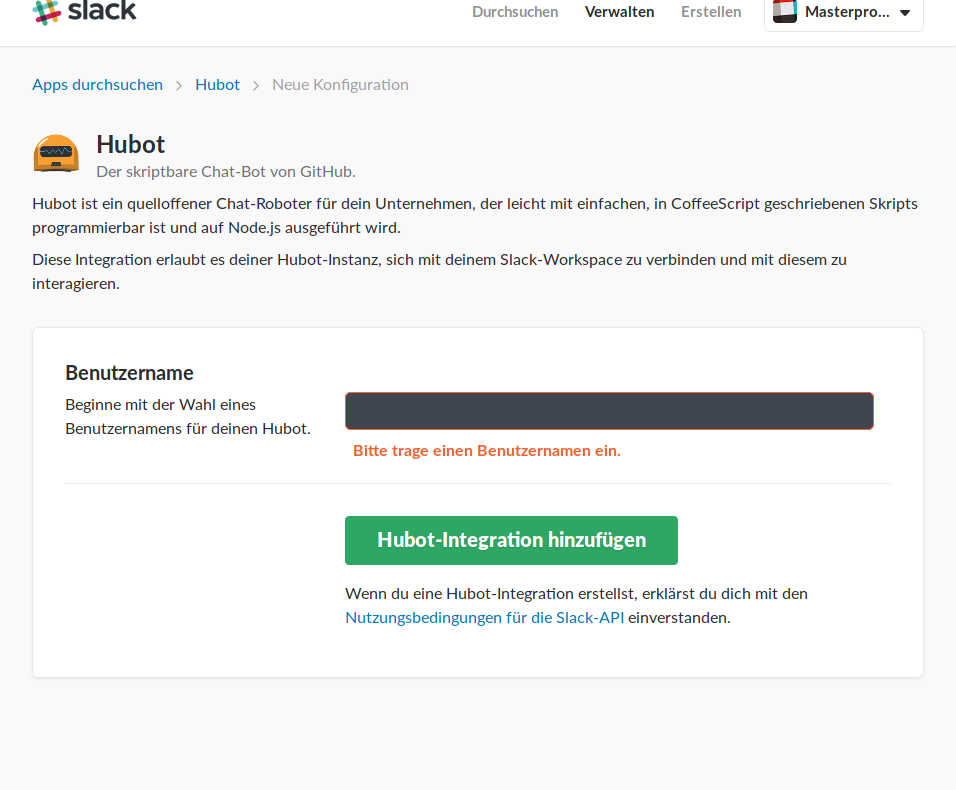
\includegraphics[width=0.8\textwidth]{img/hubot-int.png}
    \caption{Seite zum Anlegen einer neuen Bot-Konfiguration}
    \label{img:hubot-int}
\end{figure}

\subsection{Starten der lokalen Umgebung}
Nach Abruf des Projekts (über \verb+git clone+ oder Herunterladen des Archivs) befindet sich der Quellcode im Ordner \textit{docker} mit folgenden Dateien:\footnote{\url{https://github.com/ohli/steckerbot}}

\begin{verbatim}
bin/
db-data/
node_modules/
scripts/
abfragen.sql
docker-compose.yml
Dockerfile
external-scripts.json
generate_config.sh
package.json
\end{verbatim}

Die Umgebung wird dynamisch aus zwei Docker-Containern aufgebaut, welche mittels docker-compose verknüpft werden. Alle vom Standard abweichenden Einstellungen werden über die \texttt{steckerbot.env} definiert. Diese kann über den Aufruf der \texttt{generate\_""config.sh} generiert werden. Beim Aufruf wird automatisch ein Passwort für den MySQL-Rootnutzer erzeugt sowie weitere Umgebungsvariablen gesetzt. Dies ist nur für Testzwecke vorgesehen und kann im produktiven Betrieb durch ein selbst gewähltes Passwort ersetzt werden. Aktuell liegen die Passwörter im Klartext in der .env-Datei vor, was durch den Einsatz von z.B. Docker Secrets\footnote{\url{https://docs.docker.com/engine/reference/commandline/secret/}} vermieden werden sollte.

\subsection{Anpassen der Umgebungsvariablen}

\subsection{Beispielbefehle}

\subsection{Besonderheiten \& Best Practices}
